%! TeX root = thesis.tex
\chapter{Evaluation}\label{sec:eval}
\IMRADlabel{results}
% Yes, i realize the chapter is "evaluation" and the IMRAD label is "results"
\section{Testing Setup}
% \subsection{Test Model Sources}
To test the algorithm developed, a collection of test meshes was sought.
The very early days of development relied on the default cube in Blender with varied mesh density.
Once Watershed segmentation yielded plausible results from the default cube, meshes from scanned objects were demanded.
To meet this request models were scoured from Fraunhofer IGD's own collection of scanned and reconstructed cultural artifacts.
Although useful to push the limits of the methods developed, cultural artifacts are not representative of the intended target objects: scrapped metal components.
All but one of the reconstructed meshes were too complex to be useful during testing.
To ensure the algorithm's generalizability additional test models were eventually sought, this time from CAD databases.
The vast majority of these came originally from Thingiverse, an online platform for users to post their 3D printable models~\cite{Thingiverse}.
The full list of test models and their sources can be found in Appendix~\ref{app:model_table}.

\subsection{Remeshing}
Because Watershed segmentation requires input models to have a mesh of vertices upon which the height function may be computed, and CAD models store only what is required to reconstruct their geometry, remeshing was required as a pre-processing step.
PyMeshLab's ``isotropic explicit remeshing'' was chosen for this purpose~\cite{PyMeshLab}.
Manually varying the mesh density by model region can reduce mesh file sizes and expedite computation time without compromising the quality of the path planned, but is still typically slower than applying a high-density mesh to the entire model and accepting slower algorithm completion times.
The primary input parameter of \textit{isotropic explicit remeshing} is the ``target length'', which sets the target length of the remeshed edges as a percentage of ``something''.
Unfortunately PyMeshLab's documentation is unclear as to what this value is a percentage of.
% I tried to find the answer, believe me.
The vast majority of test models were remeshed with a uniform ``target length'', and the remainder were remeshed using manual selection of regions.
Models that were remeshed with non-uniform target lengths have a range of values in the \textbf{Mesh} column in appendix \ref{app:model_table}.

Prior to testing each test object was examined and assigned a ``difficulty class'' from 1-4.
The difficulty classification was created during a period when the algorithm's conic regression and cylinder detection functionality were sub-optimal and required improvement.
Hence the higher difficulty class for objects with cylindric surfaces.
The example images in the following sections were created using Blender~\cite{Blender}.

\subsection{Difficulty Class 1}
These objects are comprised solely of planar surfaces and should pose little to no trouble to the path planner.
Figure \ref{fig:class_1_models} shows 3 such examples.

\begin{figure}[htb]
\centering
\begin{subfigure}{0.3\textwidth}
	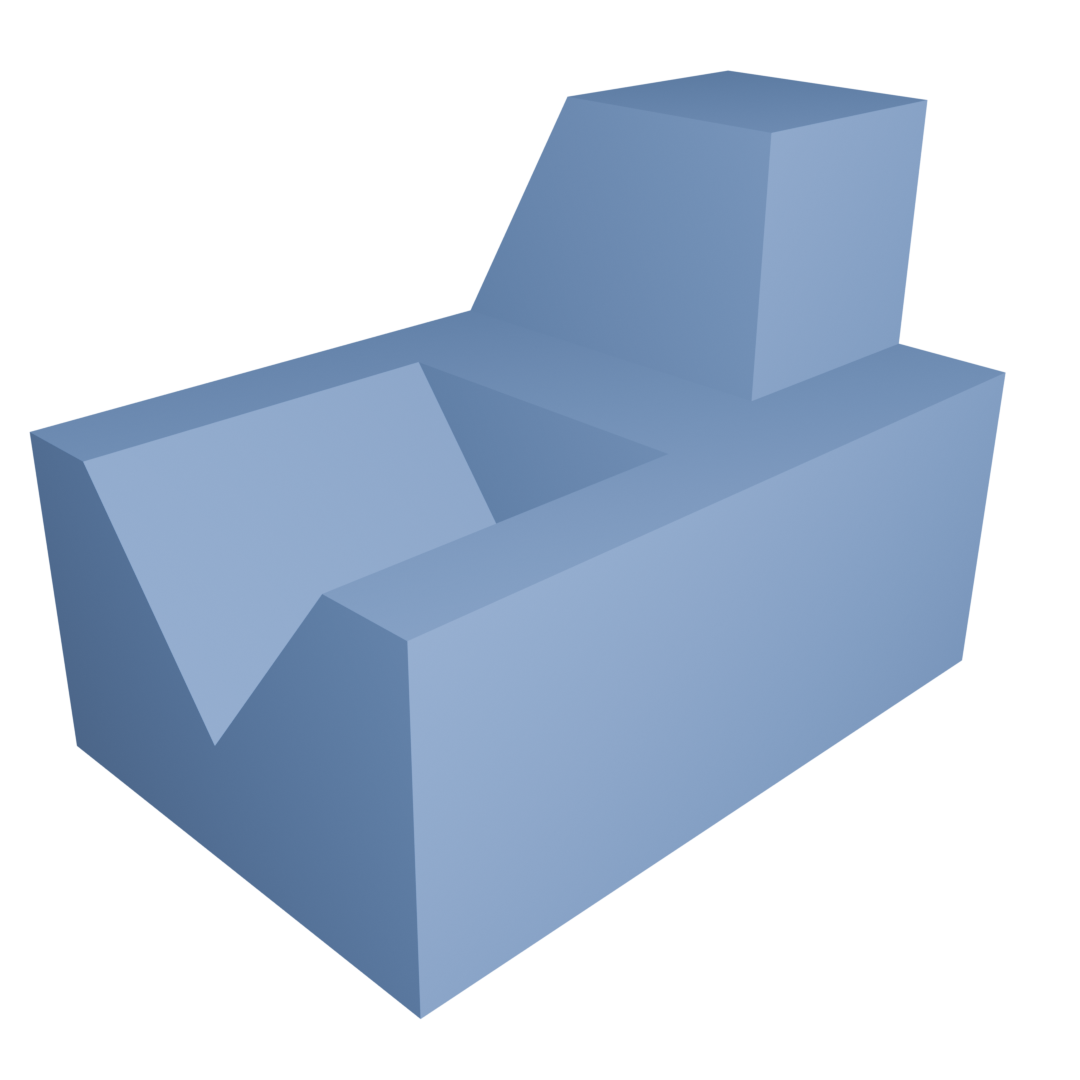
\includegraphics[width=\textwidth]{../resources/models/fc028.png}
	\caption{Model fc028}
	% \label{sfig:first}
\end{subfigure}
\hfill
\begin{subfigure}{0.3\textwidth}
	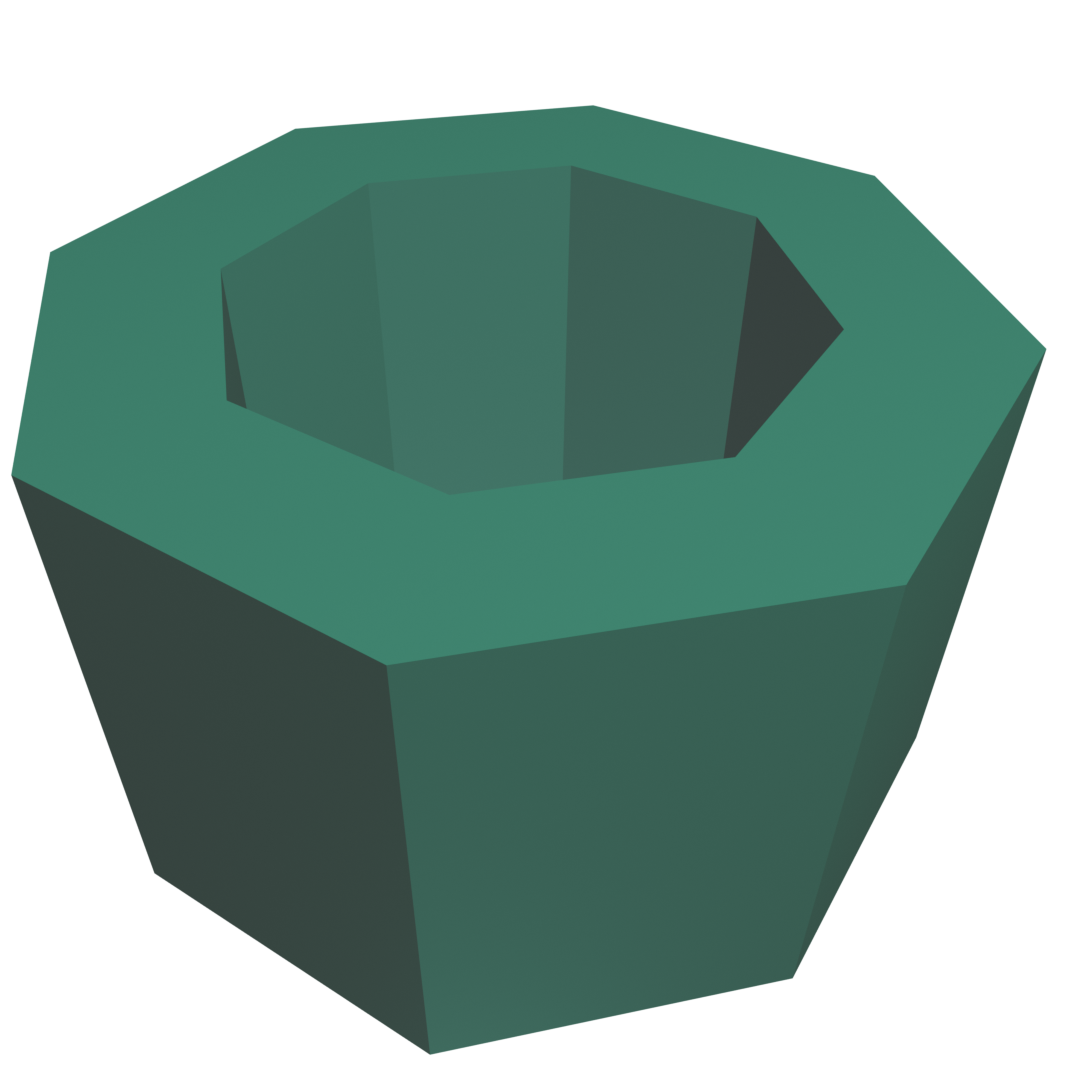
\includegraphics[width=\textwidth]{../resources/models/1505020.png}
	\caption{Model 1505020}
	% \label{sfig:second}
\end{subfigure}
\hfill
\begin{subfigure}{0.3\textwidth}
	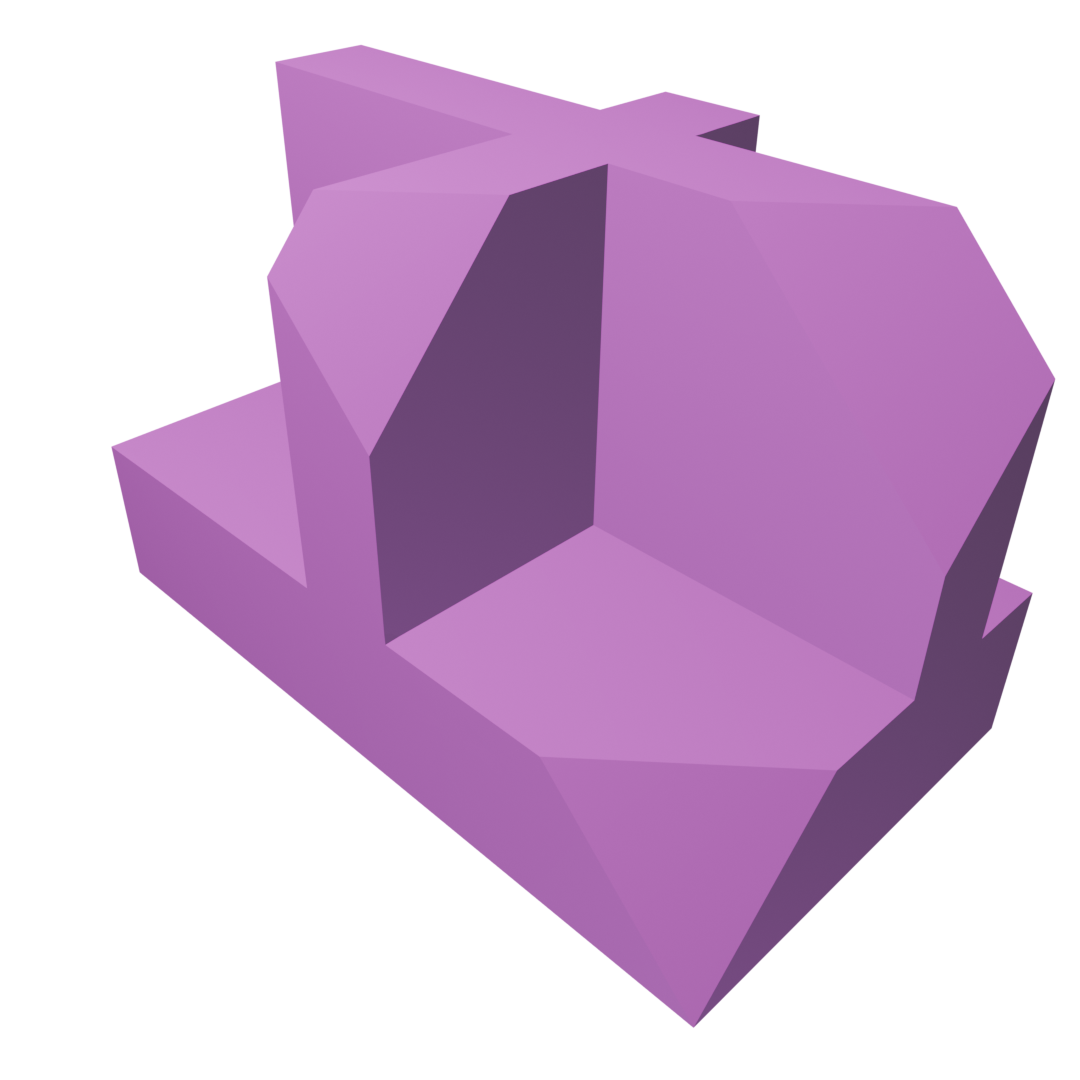
\includegraphics[width=\textwidth]{../resources/models/fc004.png}
	\caption{Model fc004}
	% \label{sfig:third}
\end{subfigure}
\caption{Test models of difficulty class 1}
\label{fig:class_1_models}
\end{figure}

\subsection{Difficulty Class 2}
Features that would cause an object to be pushed into class 2 include small or narrow surfaces, as well as cylindric surfaces.
There is a decent chance that small and thin surfaces will be absorbed into a neighboring large planar region, decreasing the chance that the combined region will be classified as planar.
Three examples of class 2 test models can be found in Figure \ref{fig:class_2_models}.

\begin{figure}[htb]
\centering
\begin{subfigure}{0.3\textwidth}
	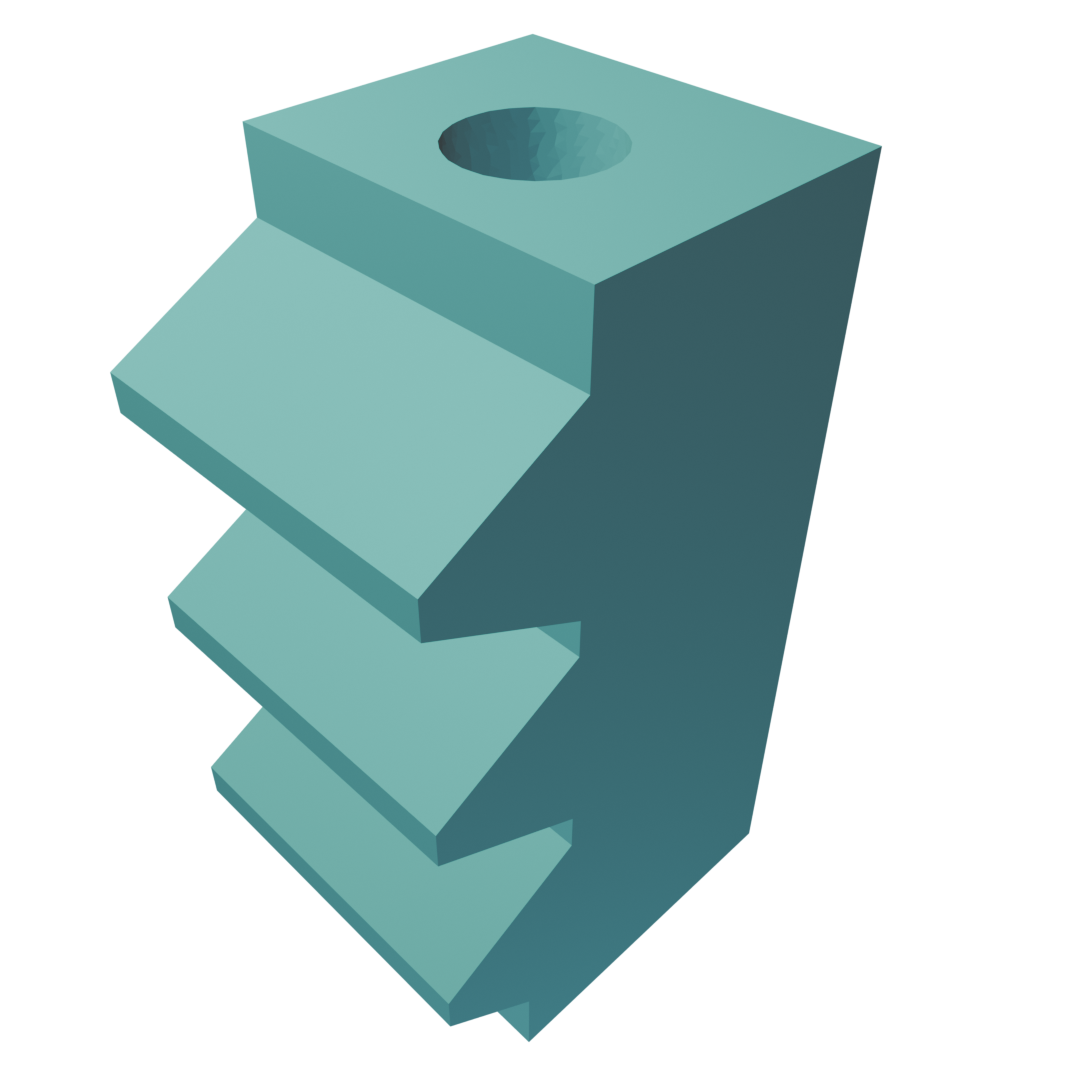
\includegraphics[width=\textwidth]{../resources/models/55583.png}
	\caption{Model 55583}
	\label{sfig:55583}
\end{subfigure}
\hfill
\begin{subfigure}{0.3\textwidth}
	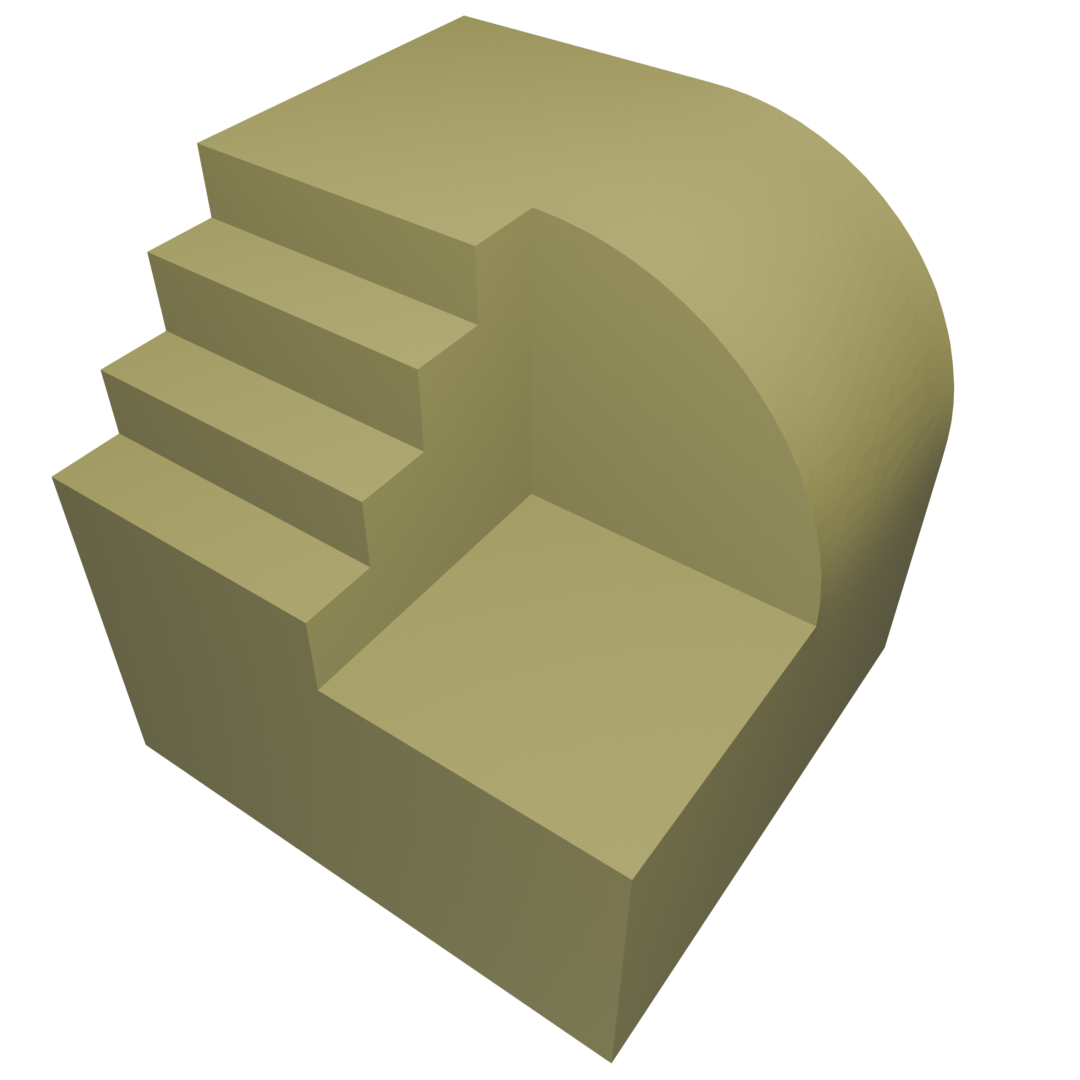
\includegraphics[width=\textwidth]{../resources/models/7120369.png}
	\caption{Model 7120369}
	\label{sfig:7120369}
\end{subfigure}
\hfill
\begin{subfigure}{0.3\textwidth}
	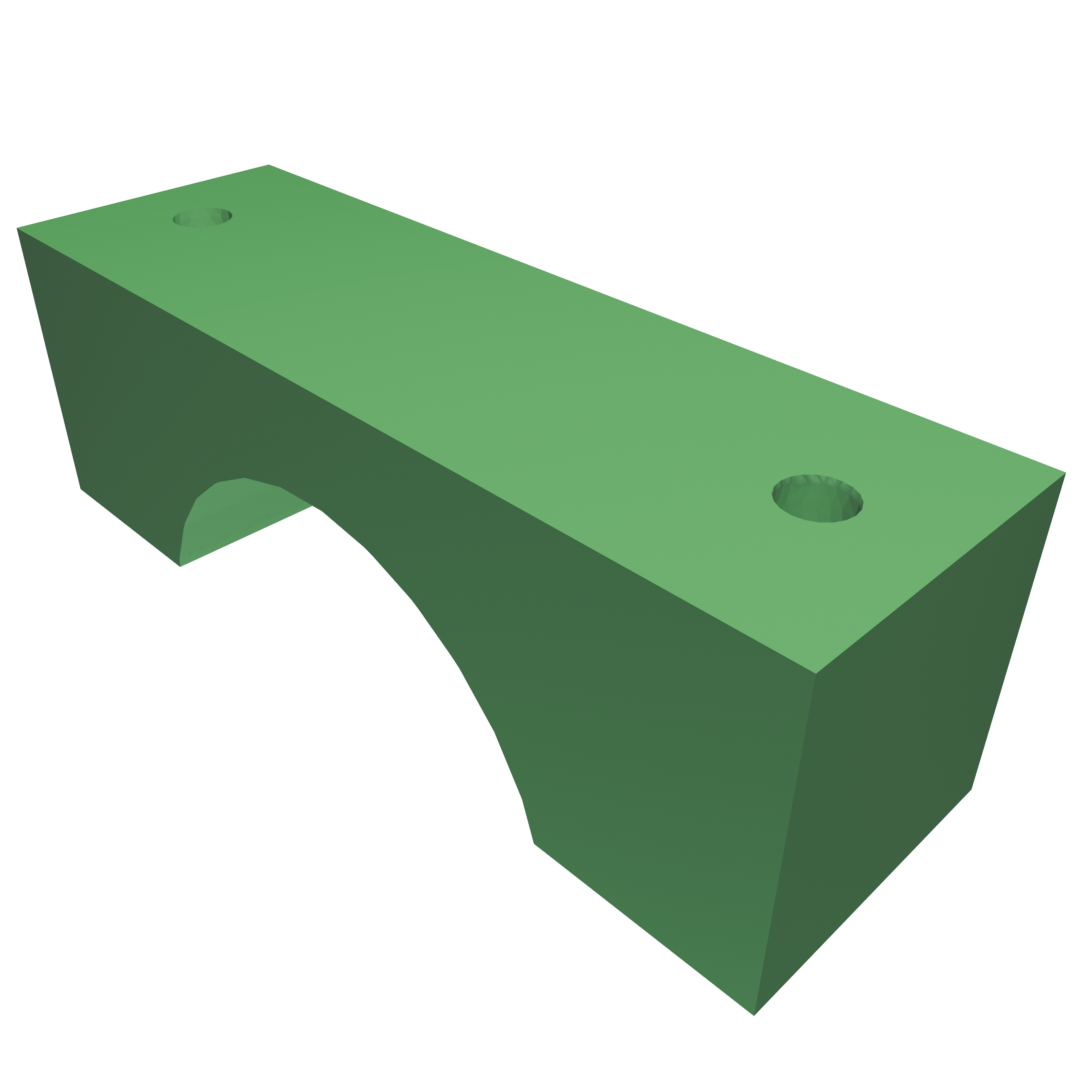
\includegraphics[width=\textwidth]{../resources/models/68501.png}
	\caption{Model 68501}
	% \label{sfig:third}
\end{subfigure}
\caption{Test models of difficulty class 2}
\label{fig:class_2_models}
\end{figure}

Of the models shown in Figure \ref{fig:class_2_models} model 55583 (Figure \ref{sfig:55583}) has the highest potential for failure, due to the narrow surfaces at the top of each gear tooth.
The smooth transitions from planar to cylindric in Figure \ref{sfig:7120369} will also be difficult for the path planner.

\subsection{Difficulty Class 3}
Objects of this class are expected to be difficult despite improvements to cylinder detection and regression, and handling of narrow planar surfaces.
The examples shown in Figure \ref{fig:class_3_models} showcase various difficult features.

\begin{figure}[htb]
\centering
\begin{subfigure}{0.3\textwidth}
	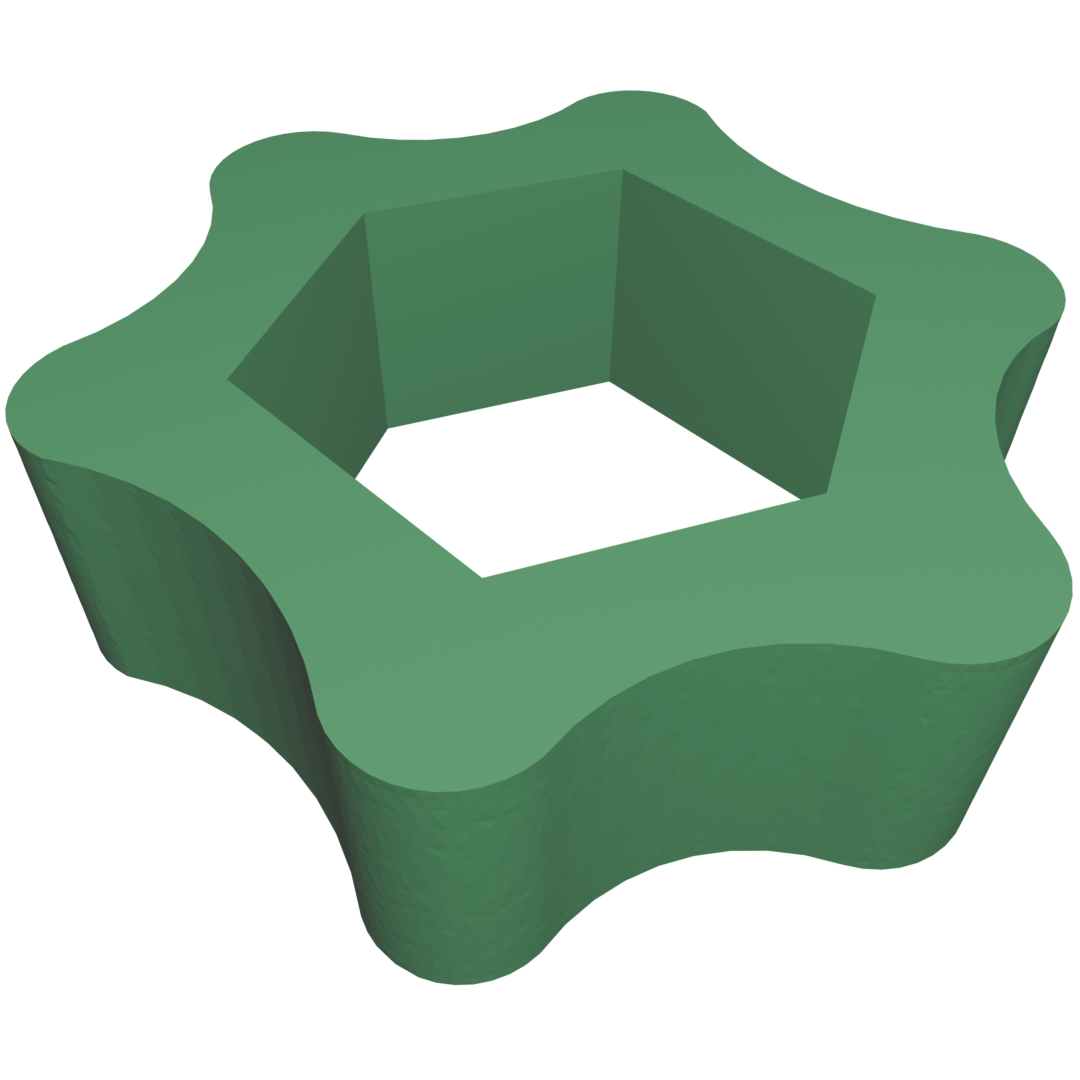
\includegraphics[width=\textwidth]{../resources/models/97733.png}
	\caption{Model 97733}
	% \label{sfig:first}
\end{subfigure}
\hfill
\begin{subfigure}{0.3\textwidth}
	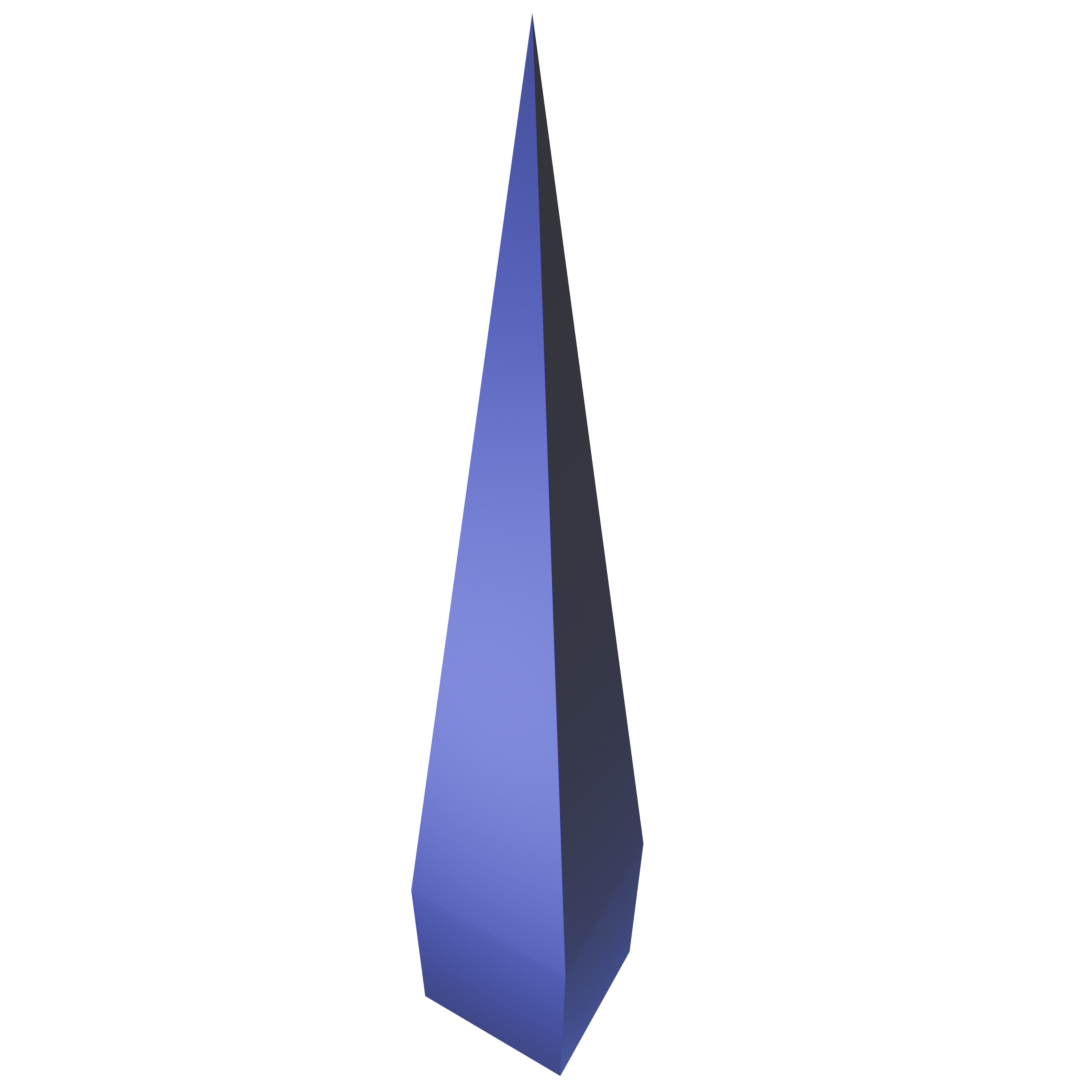
\includegraphics[width=\textwidth]{../resources/models/42042.png}
	\caption{Model 42042}
	% \label{sfig:second}
\end{subfigure}
\hfill
\begin{subfigure}{0.3\textwidth}
	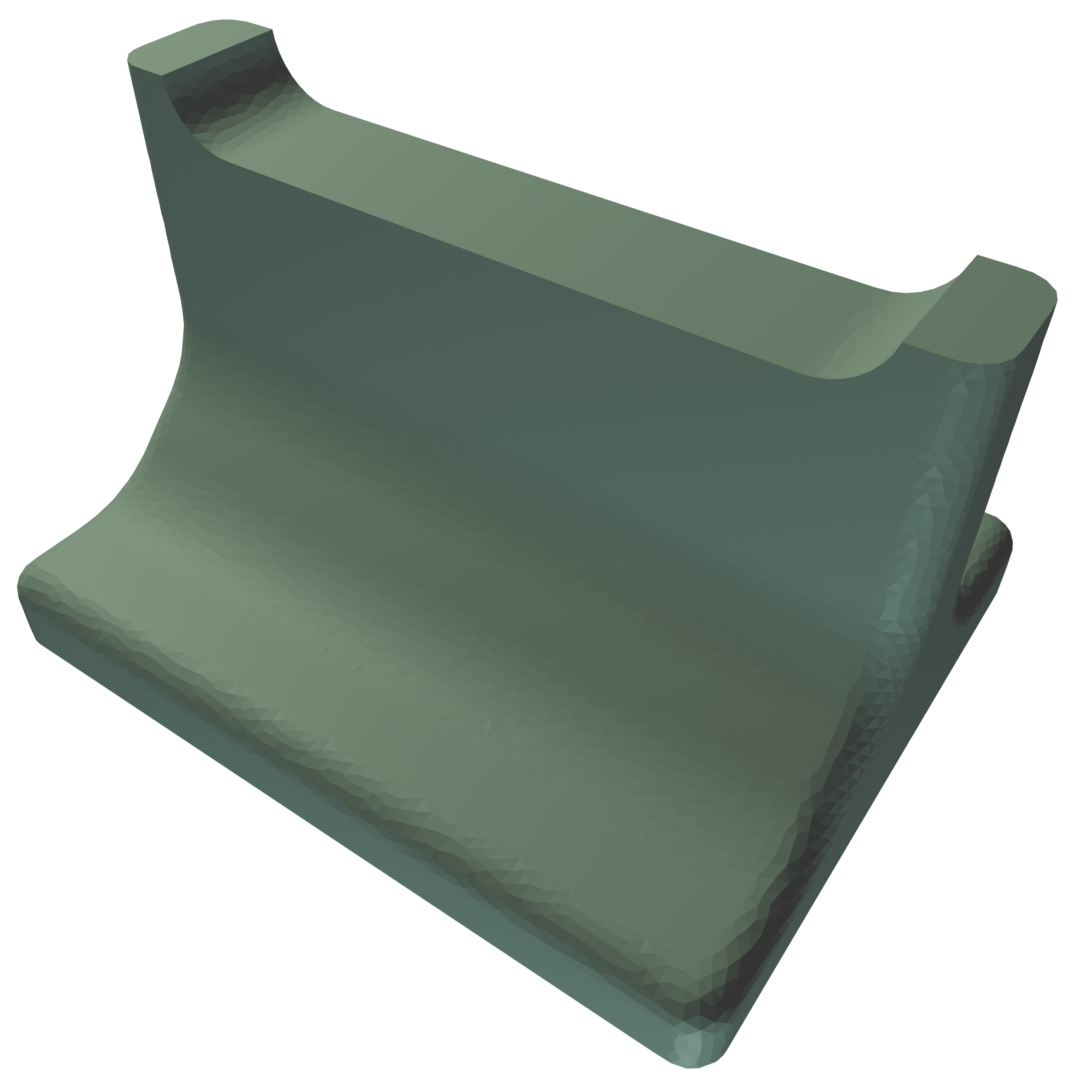
\includegraphics[width=\textwidth]{../resources/models/1148449.png}
	\caption{Model 1148449}
	% \label{sfig:third}
\end{subfigure}
\caption{Test models of difficulty class 3}
\label{fig:class_3_models}
\end{figure}

\subsection{Difficulty Class 4}
Difficulty class 4 models are beyond the scope of this work, but are included for comparison purposes.
Figure \ref{fig:class_4_models} shows a few such models.

\begin{figure}[htb]
\centering
\begin{subfigure}{0.3\textwidth}
	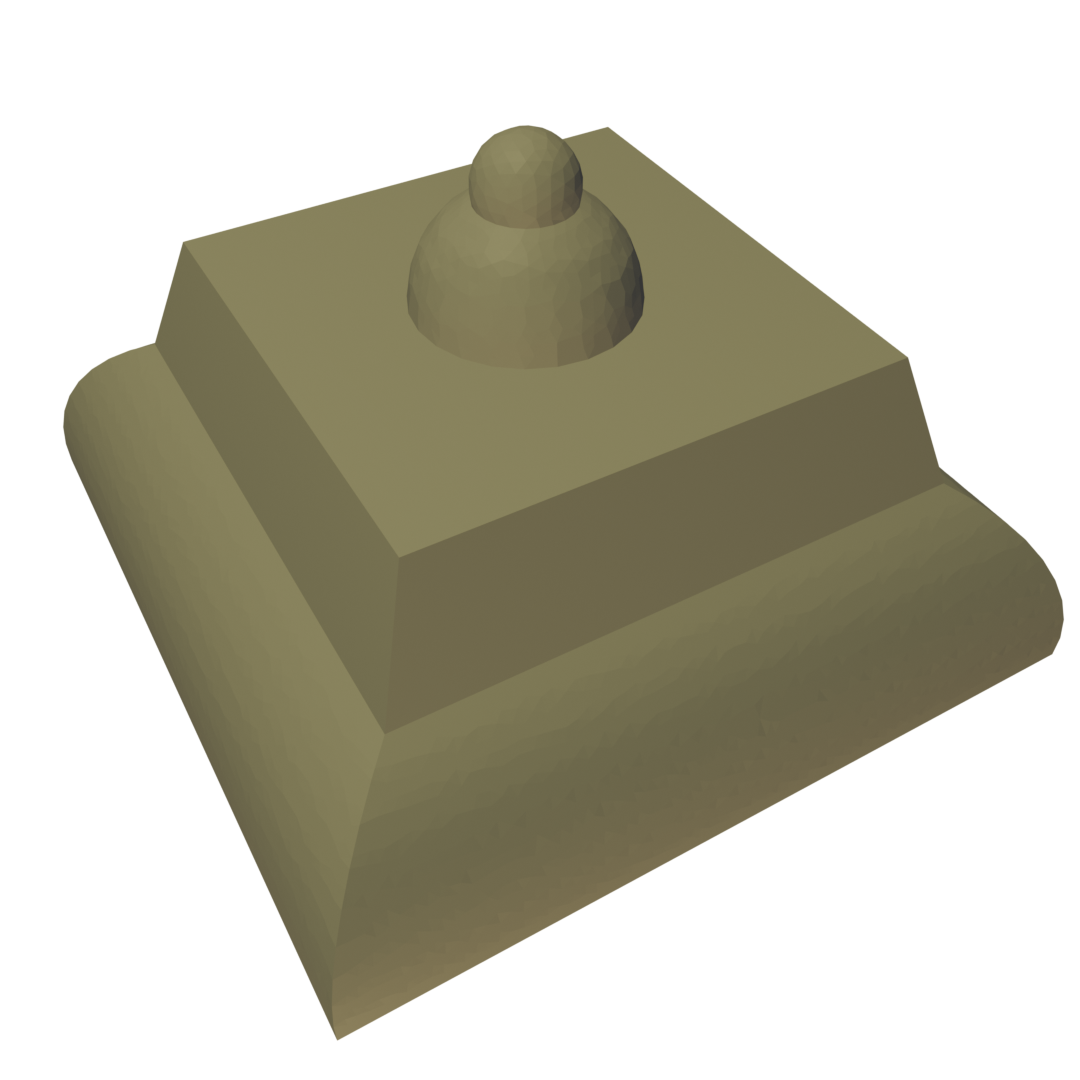
\includegraphics[width=\textwidth]{../resources/models/50704.png}
	\caption{Model 50704}
	\label{sfig:50704}
\end{subfigure}
\hfill
\begin{subfigure}{0.3\textwidth}
	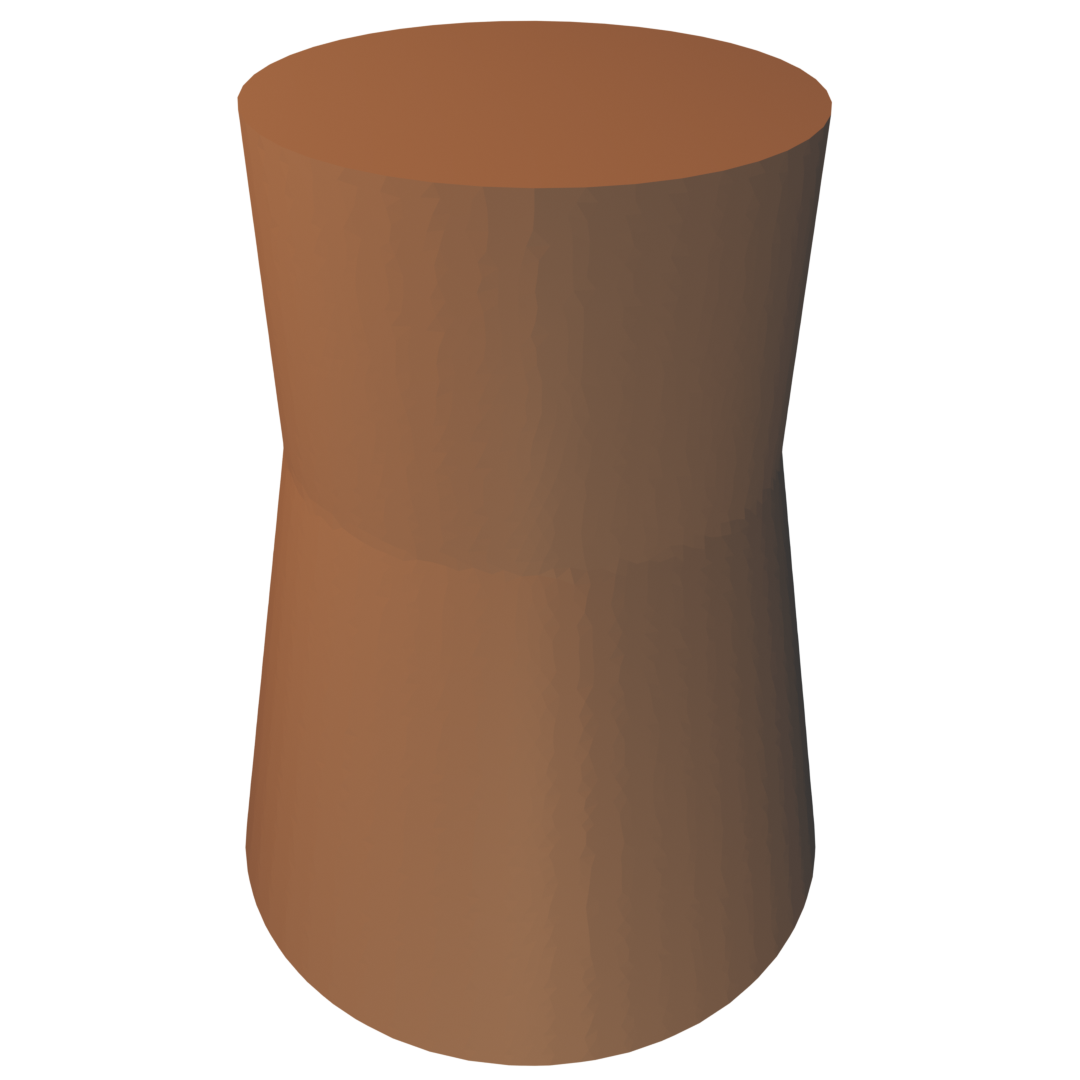
\includegraphics[width=\textwidth]{../resources/models/229605.png}
	\caption{Model 229605}
	\label{sfig:229605}
\end{subfigure}
\hfill
\begin{subfigure}{0.3\textwidth}
	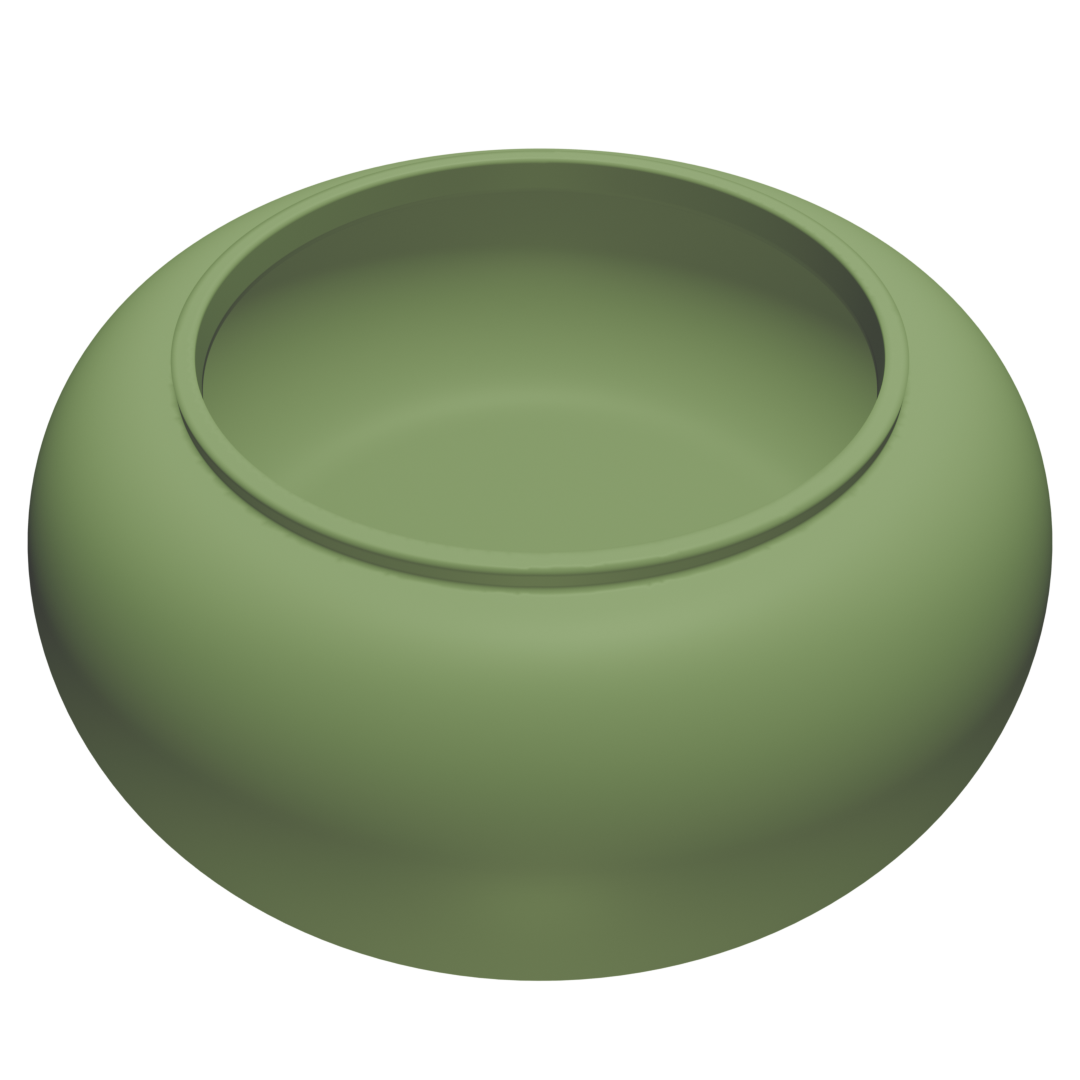
\includegraphics[width=\textwidth]{../resources/models/99265.png}
	\caption{Model 99265}
	\label{sfig:99265}
\end{subfigure}
\caption{Test models of difficulty class 4}
\label{fig:class_4_models}
\end{figure}

Although spherical surfaces, such as those adorning model 50704 (Figure \ref{sfig:50704}), were part of the planned set of detectable primitives, that functionality was not completed.
Thus, even if the path planner were able to perfectly handle the curved surfaces at the base of model 50704, the partial spheres would result in a failure.
Model 229605 (Figure \ref{sfig:229605} appears simple at first glance, but its lower half is that of a cone, and the detection thereof is not implemented.
Model 99265, shown in Figure \ref{sfig:99265}, exhibits swept curves which the path planner is unable to process.
Its overall form, comprised of occluded regions, is also beyond the scope of the intended application of the path planner developed.


\section{Results}
A test is considered a success if the path planning algorithm completes without error and a visual inspection confirms the paths planned.
If an error is thrown or if the paths planned deviate noticeably from the model's surfaces, the test is a failure.
Of the 18 class 1 models, paths were successfully planned on 12.
Paths were unable to be planned on the remaining models.
The paths planned from 2 of the 12 successes are shown in Figure~\ref{fig:class_1_results}.

\begin{figure}[htb]
	\centering
	\begin{subfigure}{0.4\textwidth}
		\includegraphics[width=\textwidth]{../resources/models/91142_paths.png}
		\caption{Model 91142 paths}
		% \label{sfig:91142_paths}
	\end{subfigure}
	\hfill
	\begin{subfigure}{0.4\textwidth}
		\includegraphics[width=\textwidth]{../resources/models/1505020_paths.png}
		\caption{Model 1505020 paths}
		\label{sfig:1505020_paths}
	\end{subfigure}
	\caption{Paths planned for class 1 models}
	\label{fig:class_1_results}
\end{figure}

Close inpsection of the paths shown in Figure~\ref{fig:class_1_results} reveals that the paths are disconnected from one another.
This is because the TSP solver was cut from the scope of this project.
Due to the octagonal hole in model 1505020 (see Figure~\ref{sfig:1505020_paths}) the top and bottom faces were segmented into 8 sub-regions during the \textit{Interior Edge Extension} step.
The full list of models, outcomes, and a brief explanation of the cause of failure can be found in Appendix \ref{app:model_table}.

